\begin{comment}
  \bibliography{project.bib}
\end{comment}

\chapter{IM -- The General Image Format}
\label{cha:im}

\begin{refsection}

  \section{Introduction}
  \label{sec:introduction}

  In this chapter, we are to explore an imaginary image format called
  \textit{IM}\index{IM}. By studying this extremely simple image format, we will get a good
  general view of how image formats are structured.

  But before we dive in, let me clarify one thing for you: all data that
  is stored in a computer is just a sequence of numbers. How this
  sequence of numbers is to be parsed is defined by it's \textit{file
    format} \index{file format}. The entirerity of a file format is
  specified in its \textit{specification}\index{specification}.

  \section{The IM Image Format}
  \label{sec:general-image-format}

  \begin{figure}
    \centering
    \inputtikz{im_format.tex}
    \caption{IM image format}
    \label{fig:im}
  \end{figure}

  Observe figure \ref{fig:im}. It demonstrates a picture of a pretty
  flower in the imaginary file format IM\index{IM}. It nicely
  demonstrates the elements common to all image formats. Let's go
  through them one by one:

  \subsection{Image Header}
  \label{sec:image-header}

  The first numbers of an image is always its image header\index{image
    header}. How many numbers it consists of is specific to the image
  format in question. The image header gives general information about
  an image that greatly helps the loading process. It usually includes
  information like the width, height and color depth of the image.

  \subsubsection{Magic Numbers}
  \label{sec:magic-numbers}

  Let's look at our example image. The first two number is the two
  ASCII letters IM. These numbers are known as magic numbers
  \index{magic numbers}. You see, at the beginning of every image
  file, there a couple bytes called magic numbers that are common to
  all images of that type. They are sort like file name extensions,
  meaning that they help you identify the type of the file you are
  currently reading.

  \subsubsection{Measurements}
  \label{sec:measurements}

  And following the magic number is the width and the height of the
  image. In practically every image format this information is
  included.

  \subsection{Color Palette}
  \label{sec:color-pallete}

  Color palettes \index{color palette} are also very common, but not
  all images out in the wild use them, but as good all image formats support
  them, hence why they are included in this imaginary format. A color
  palette is basically an array or list of colors that is to be used
  by the image.

  \subsection{The Color Data}
  \label{sec:color-data}

  Following the header and the optional color palette is the actual
  color data. Now let us talk about how the colors are stored as an
  image.

  An image is simply a grid of colors. As demonstrated in figure
  \ref{fig:im}. As you can
  see, an image really only consists of a lot of tiny,tiny little
  colored squares. We usually refer to these squares as pixels
  \index{pixel}. (todo{cite sources})

  So as we can see from our sample image format, IM, the flower image
  is just a couple of colored pixels. But in this case a color palette
  is used. This means the image indexes the color palette like an
  array or list. So instead of the image containing its actual color,
  it in this case just contains a bunch of index numbers.

  If a color palette were not to be used in this case, the image would
  just contain a grid of raw colors.

  The color stored in an image and/or palette uses a certain bit
  depth, as we discussed in chapter \ref{cha:color}. This information
  is almost \textit{always} included in the image format. I didn't
  specify a color depth for this format to keep the example simple and
  understandable.

  \section{Done\dots?}
  \label{sec:done}

  But it's not really that simple. A majority of all image format have
  had some sort of compression applied to their color data. And
  performing the decompression of that image data is usually the
  most difficult part, unfortunately.

  But why would you even need compression?  Because it just isn't
  feasible to just store the color data uncompressed. Sometimes
  there's literally millions of pixels in an image. Photgraphies are
  an example of this, like for example figure \ref{fig:flowers}.

  Not even for images with very simple and non varying color data like
  logos is this method good for. Look at for example at the logo
  \ref{fig:logo} It doesn't do try to find the very similar color data
  and do compression. Even a very,very simple compression algorithms
  can do wonder on an image such as the logo,  cutting down the size by
  maybe even by a half!

  Thus, in the next chapter we are to explore compression algorithms
  commonly used in image formats.

  \todo{motivate and explain how much the filesize increases by
    providing examples using NetPBM}

  \begin{figure}
    \centering
    \newcommand{\shieldcolor}{red}
    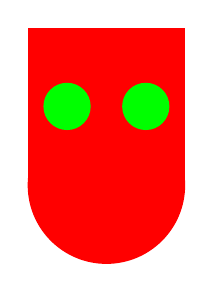
\begin{tikzpicture}
      \fill[\shieldcolor] (0,0) rectangle (2,2);
      \fill[\shieldcolor] (1,0) circle (1);

      \fill[green] (0.5,1) circle (0.3);
      \fill[green] (1.5,1) circle (0.3);

    \end{tikzpicture}
    \caption{Exemplary logo.}
    \label{fig:logo}
  \end{figure}

  \begin{figure}
    \centering
    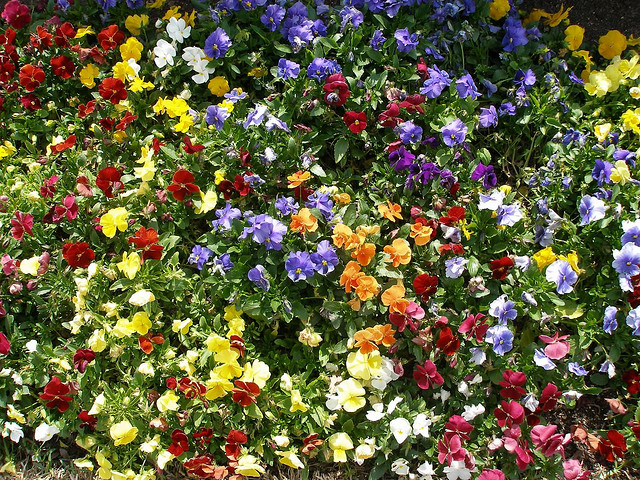
\includegraphics[scale=0.05]{tikz_img/flowers.jpg}
    \caption{Flowers \cite{turner06:_flower}.}
    \label{fig:flowers}
  \end{figure}

  \FloatBarrier

  \printbibliography[heading=subbibliography]

\end{refsection}